\documentclass[12pt,a4paper,english]{amsart}
\usepackage{graphicx}
% \usepackage{algorithm}
% \usepackage{algorithmic}
\makeatletter  
\newif\if@restonecol  
\makeatother  
\let\algorithm\relax  
\let\endalgorithm\relax  
\usepackage[linesnumbered,ruled,vlined]{algorithm2e}
\usepackage{algpseudocode}
\usepackage{hyperref}
\usepackage{lineno}
\usepackage[a4paper, top=2.8cm, left=2cm, right=2cm, bottom=2cm]{geometry}
%\linenumbers
\renewcommand{\algorithmicrequire}{\textbf{Input:}}  % Use Input in the format of Algorithm  
\renewcommand{\algorithmicensure}{\textbf{Output:}} % Use Output in the format of Algorithm 
% ----------------------------------------------------------------
\vfuzz2pt % Don't report over-full v-boxes if over-edge is small
\hfuzz2pt % Don't report over-full h-boxes if over-edge is small
% ----------------------------------------------------------------
\begin{document}

\title{Case Study - Disk Failure Prediction}%
\author{Wei Ren}%
%\email{mathvivi@hotmail.com}%
%\subjclass{}%
\keywords{Machine Learning, SMART, Disk Failure}%

\date{\today}
%\dedicatory{}%
%\commby{}%
% ----------------------------------------------------------------
\begin{abstract}
  The motivation of this report is to show a case study of disk failure prediction as a coding test/supporting material for the application of an AIOps position of Alibaba Group.
  In this report, the detailed illustration of data preprocessing and feature engineering, model choosing and parameter tuning, results evaluation and insights from this task are included.
\end{abstract}
\maketitle
%\tableofcontents{}
% ----------------------------------------------------------------
\section{Brief Introduction}

\subsection{Introduction}

Various disk failures are not rare in large-scale IDCs and cloud computing environments, fortunately, we have S.M.A.R.T. (Self-Monitoring, Analysis, and Reporting Technology; often written as SMART) logs collected from computer hard disk drives (HDDs), solid-state drives (SSDs) and eMMC drives that detects and reports on various indicators of drive reliability, with the intent of enabling the anticipation of hardware failures.

In data center environments, hard disk drive (HDD) failures are a rare but costly occurrence. Therefore, HDD vendors are highly motivated to reduce the rate of failures as a cost saving measure. But currently, HDD manufacturers use Self-Monitoring and Reporting Technology (SMART) attributes collected during normal operations to predict failures. SMART attributes represent HDD health statistics such as the number of scan errors, reallocation counts and probational counts of a HDD. If a certain attribute considered critical to HDD health goes above  its  threshold  value,  the  HDD  is  marked  as  likely  to  fail  [P  inheiro] .
Our project focuses on applying machine learning to improve prediction accuracy over baseline heuristics in hard disk drives. The goal of our project is twofold: 1) to achieve a higher recall, precision and accuracy than our baseline implementation modeled off of current enterprise failure detection models. 2) to analyze which of our subset of machine learning models is best suited towards predicting failure of HDDs. We analyze three different algorithms: Logistic Regression, Naive Bayes and Random Forest, to see which has the highest accuracy, recall and precision when   predicting   HDD   failures.

\subsection{Literature Review}

Pinheiro et al analyzed failure trends in a large disk drive population of over one hundred thousand enterprise HDDs at a Google data center. They found that specific SMART parameters (scan errors, reallocation counts, offline reallocation counts, and probational counts) had a large impact on failure probability. Most importantly, a large fraction of failed drives showed no signs of failure in all of its monitored SMART features, making it unlikely to achieve an accurate predictive failure model that can be built based on SMART signals alone [Pinheiro]. Similarly, BackBlaze analyzed the correlation rates between its HDD failures and SMART attributes and found that SMART 5, 187, 188, 197, and 198 had the highest rates of correlation to HDD failure. These SMART attributes are also related   to   scan   error,   reallocation   count   and   probational   counts   [Klein].
Pitakrat et al evaluated 21 machine learning (ML) algorithms for predicting HDD failure. Pitakrat et al found that of the 21 ML algorithms tested, a Random Forest algorithm produced the highest area under a ROC Curve (AUC), while   a   Nearest   Neighbor   classifier   had   the   highest   F1-score.
Hughes et al also studied machine learning methods for predicting failures in HDDs. They analyzed the performance of Support Vector Machines (SVM), rank-sum and multi instance Naive Bayes. SVMs achieved the highest   performance   with   a   50.6\%   detection   and   0\%   false   alarm   rate   [Hughes   et   al].

% ----------------------------------------------------------------
%
% ----------------------------------------------------------------
\section{Data Preprocessing and Feature Engineering}

Data sources from \url{https://www.backblaze.com/b2/hard-drive-test-data.html}

As of the end of 2017, there are about 88 million entries totaling 23 GB of data. Each entry consists of the date, manufacturer, model, serial number, status (operational or failed), and all of the SMART attributes reported by that drive. 
5, 187, 188, 197, 198
\begin{algorithm}  
	\caption{Data importing and preprocessing}
	\LinesNumbered  
	\KwIn{The origianl test data of the year of 2017 plus Q4 of 2016 from Backblaze}
	\KwOut{Raw and normalized values of the five SMART attributes for the year of 2017, along with failure/operational status, date, serial number}
	($X$, $Y$) = Data selection(SMART $5$, SMART $187$, SMART $188$, SMART $197$, SMART $198$, date, serial number, Failure status)\;  
	Initialize a new column for each SMART attribute with $0$, named SMART binary, to denote if this attribute is non-zero  \;
	\If{ SMART attributes $\neq 0$ }
	{
		let the value be $1$
	}
	\If{ failure status is true}  
	{  
		Mark last $60$ days (if applicable) of the HDD's \textit{failure status as true} \;  
	}
	\textbf{return} $X$ and $Y$, with three versions (raw, normalized, binary values of SMART attributes);
\end{algorithm}  

% http://blog.csdn.net/lwb102063/article/details/53046265
% https://oeis.org/wiki/List_of_LaTeX_mathematical_symbols

There are some critical questions to be answered if one needs to complete this case study:

\begin{itemize}
	\item Define the amount of data, and which columns should be counted; Data inputs.
			Data of the year of 2017.
	\item Define the features; Some feature selection methods.
	\item Define the training data sets and test data sets; Cross-validation for model selection.
	\item Define model, cost/loss function, parameters, training methods. Machine Learning. Scikit-Learn
	\item Train the models and tune parameters.
	\item Conduct prediction for other data sets and evaluate results. Confusion Matrix.
\end{itemize}

\subsection{Data Preprocessing}


\begin{enumerate}
	\item Choose raw over normalized SMART Data points
	\item Failure status smoothing/backtracking
	\item Filter out all HDD models besides Seagate models
	\item Balance out the data set
\end{enumerate}

\subsection{Feature Engineering}

\subsubsection*{Feature Selection}

\begin{itemize}
	\item Filter
	\item Wrapper
	\item Embedded
\end{itemize}

From experience, BackBlaze have found the following 5 SMART metrics indicate impending disk drive failure:

\begin{itemize}
	\item \textbf{SMART 5: Reallocated Sector Count.} \\
	When the drive’s logic believe that a sector is damaged, it can remap the faulty sector number to a new physical sector drawn from a pool of spares.
	\item \textbf{SMART 187: Reported Uncorrectable Errors.} \\
	The count of errors that could not be recovered using hardware ECC. Large scan error counts can be indicative of surface defects and therefore are believed to be indicative of lower reliability.
	\item \textbf{SMART 188: Command Timeout.} \\
	The count of aborted operations due to HDD timeout.
	\item \textbf{SMART 197: Current Pending Sector Count.} \\
	Disk drives put suspect bad sectors on probation until they either fail permanently and are reallocated or continue to work without problems.
	\item \textbf{SMART 198: Offline Uncorrectable.} \\
	The total count of uncorrectable errors when reading/writing to a sector. A rise in the value of this attribute indicated defects of the disk surface and/or problems in the mechanical subsystem.
\end{itemize}

Ninety variables and millions of data points not only take an extensive amount of time to train and test on, but can also lead to overfitting. To reduce the computational workload and improve the performance of our models, we chose   to   select   only   the   most   relevant   features   and   avoid   features   with   a   large   amount   of   unfilled   data   points.
% ----------------------------------------------------------------
%
% ----------------------------------------------------------------
\section{Model Selection and Parameters Tuning}

How to choose machine learning models and tune the parameters?

Reduce to a classification problem.

\begin{algorithm}  
	\caption{Model selection, training, and parameters tuning}
	\LinesNumbered  
	\KwIn{$X$ and $Y$ of the year of 2017}
	\KwOut{Trained model}
	Split the datasets into two pieces, training datasets ($X_{train}$, $Y_{train}$) and validation datasets ($X_{test}$, $Y_{test}$), by cross validation\;
	Train different models with training datasets\;
	\Repeat{parameters are optimized or maximum iterations exhausted}
	{
		Evalute the models and tune parameters\;
	}
	\textbf{return} trained model;
\end{algorithm}  

\subsection*{Base Line}

Our baseline analysis mimics what BackBlaze currently implements in its failure prediction system. We analyze five SMART attributes ( SMART 5, 187, 188, 197, 198) and predict a HDD will fail if any of these critical raw SMART   attributes   are   greater   than   0.
Our goal is therefore to maintain as high of a TPR with a maximum TPR equal to the baseline analysis, and to focus   on   reducing   the   FPR   to   0.

\subsection*{Logistic Regression}

Logistic Regression is one of the basic tools for performing binary classification. One of the assumptions made in order for Logistic Regression to potentially perform well is that the data is linear. This means that the score we obtain from Logistic Regression is affected proportionally to changes in the feature values in a linear fashion. The tool mainly served as a second baseline in some sense as it was our first attempt at the classification problem beyond implementing   the   simple   baseline.   We   also   employed   L2   regularization.

\subsection*{Naive Bayes}

The Naive Bayes classifier model makes the assumption that the value of a feature is conditionally independent of the value of another feature given some class label. Among the different techniques used for building Naive Bayes models, we chose Multinomial Naive Bayes, which assumes that the probability of a feature value given some class label   is   sampled   from   a   multinomial   distribution.   For   regularization,   we   use   Laplace   smoothing.

\subsection*{Random Forest}

Random forest is an ensemble tool which takes a subset of observations and a subset of variables to build a group of decision trees. It builds multiple such decision trees and amalgamate them together to get a more accurate and stable prediction.

\subsection*{K-Nearest Neighbours}

\subsection*{Support Vector Machines}

\subsection*{Neural Network}

% ----------------------------------------------------------------
%
% ----------------------------------------------------------------
\section{Results Evaluation}

How to evaluate the results?

To evaluate the classifier's performance, we measure precision, recall and F-score as defined below.
\begin{itemize}
	\item Precision: to measure the ability of the classifier to correctly identify disks at risk;
	\item Recall: to measure the classifier's sensitivity. A higher recall is equivalent to minimizing the number of false negatives;
	\item $F_1$ score: the combined score between precision and recall, or the weighted harmonic mean;
	\item ROC: Receiver Operating Characteristic, is the plot of TPR vs FPR. In usual, we can also draw the Precision-Recall Curve.
\end{itemize}

\begin{equation}
	P = \dfrac{TP}{TP+FP} \quad\quad 
	R = \dfrac{TP}{TP+FN} \quad\quad 
	F_{1}\; score = \dfrac{2PR}{P+R}
\end{equation}
where $TP$ refers to true positives, $FP$ is false positives and $FN$ denotes false negatives.

\begin{table}
	\caption{Confusion Matrix}
	\centering
	\begin{tabular}{|c|c|c|c|}
		\hline
		& actual positive & actual negative & total \\
		\hline
		predicted positive & $TP$ & $FP$ & $TP+FP$ \\
		\hline
		predicted negative & $FN$ & $TN$ & $FN+TN$ \\
		\hline
		total	&	$TP+FN$ & $TN+FP$ & \\
		\hline
	\end{tabular}
\end{table}

\begin{figure}[htb]
	\centering
	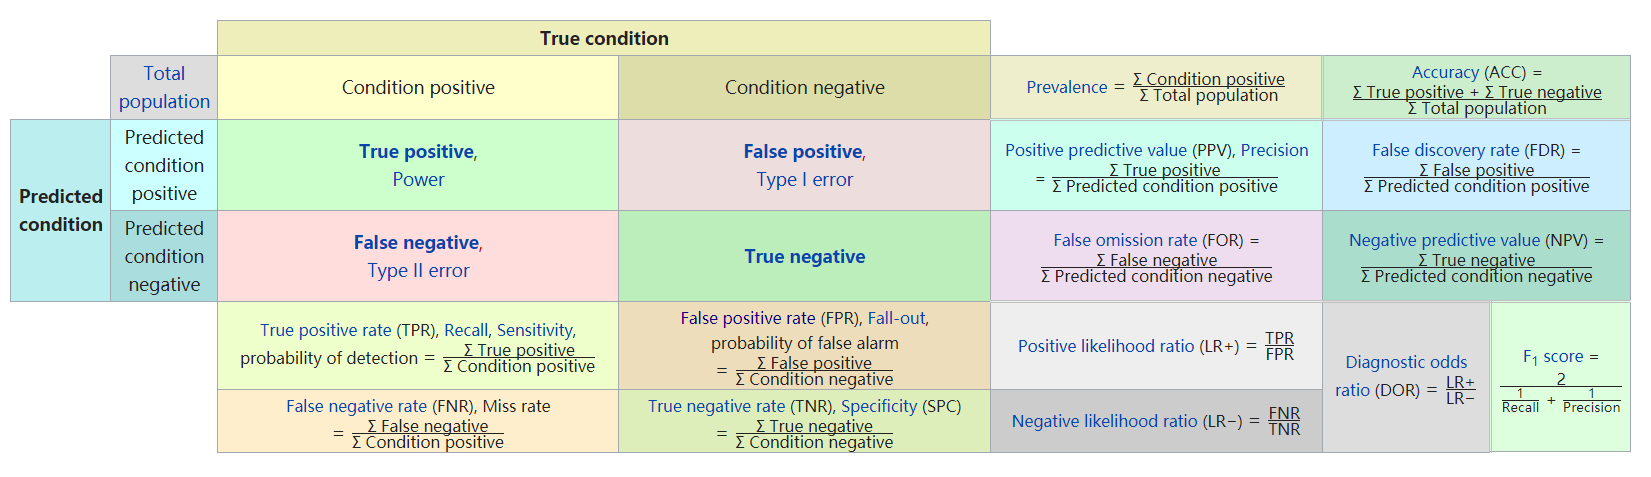
\includegraphics[width=\textwidth]{img/auc.PNG}
	\caption{Confusion Matrix\cite{Wiki}}
\end{figure}
% ----------------------------------------------------------------
%
% ----------------------------------------------------------------
\section{Conclusions}

What insights or lessons learned from this task?
\cite{Ren2018a}

% ----------------------------------------------------------------
\bibliographystyle{amsplain}
\bibliography{smart_ml}
\end{document}
% ----------------------------------------------------------------
